%% IMPORTANT: Once working, run latex 3 times to get listoffigures to work

%% Be sure to check spelling!

%% Put **your** name and the proper due date in place

%% Copy the lstlisting and figure code as many times as you need
%% Be sure to put in your own file names if appropriate

%% Note that the \epsfig command is currently commented out - until the
%%%% files exist, processing this code without them will result in an error
%%%% so leave the comments until you have created the graphics files!

\documentclass{article}
\usepackage{amsmath}    % loads AMS-Math package
\usepackage{epsfig}     % allows PostScript files
\usepackage{listings}   % allows lstlisting environment
\usepackage{moreverb}   % allows listinginput environment
\usepackage[letterpaper, margin=0.75in]{geometry}  % set paper size/margins
\usepackage{textcomp}   % adds \interrobang, among others!

\begin{document}
\begin{center}
\rule{6.5in}{0.5mm}\\~\\
\textbf{\large EGR 103L -- Fall 2017}\\~\\
\textbf{\huge Laboratory 8 - Intermediate Curve Fitting}\\~\\
**NAME (NET ID)**\\
Lab Section **NUMBER AND LETTER**, **DAY AND TIMES**\\
**DATEDUE**, **YEAR**\\~\\
{\small I have adhered to the Duke Community Standard in completing
  this assignment.  I understand that a violation of the Standard can
  result in failure of this assignment, failure of this course, and/or
  suspension from Duke University.} 
\rule{6.5in}{0.5mm}\\
\end{center}
\tableofcontents
\listoffigures
\renewcommand{\arraystretch}{1.5}
\clearpage

\section{Palm 6.9}
% Report St value
\begin{center}
\begin{tabular}{|c|c|c|c|} \hline
Order & Coefficients $P$ of $T=f(A)=\sum_{k=1}^{\mbox{Order}+1}~P(k)A^{(\mbox{Order}+1-k)}$  & $S_r$ & $r^2$ \\ \hline
1 & [] & ~ & ~\\ \hline
2 & [] & ~ & ~ \\ \hline
3 & [] & ~ & ~ \\ \hline
4 & [] & ~ & ~ \\ \hline
\end{tabular}
\end{center}
The minimum drying times and additive amounts for each fit are:
\begin{center}
\begin{tabular}{|c|c|c|} \hline
  Order & Min. Drying Time (min) & $A$ for Min. Drying
Time (oz) \\ \hline
1 & ~ & ~ \\ \hline
2 & ~ & ~ \\ \hline
3 & ~ & ~ \\ \hline
4 & ~ & ~ \\ \hline
\end{tabular}
\end{center}
% Discussion

\section{Palm 6.16}
\begin{align*}
y(x) = VALUE+VALUE~\ln(x)
\end{align*}
The statistical information is:
\begin{align*}
S_t&=VALUE & S_r &= VALUE & r^2 &=VALUE
\end{align*}
The estimates asked for using this model are:
\begin{align*}
y(2.5)&\approx VALUE & y(11)&\approx VALUE
\end{align*}

\section{Chapra 15.7}
Based on the least-squares fit of the given models,
\begin{align*}
% replace PM with + or - as appropriate
OC(c,T)&=(VALUE)PM~(VALUE)c~PM(VALUE)T~PM(VALUE)T^2~PM(VALUE)T^3
\end{align*}
For this model with these data points, 
\begin{align*}
S_t &= VALUE &
S_r &= VALUE &
r^2 &= VALUE
\end{align*}
meaning DISCUSS.  The estimate of $OC(15,12)$ is VALUE mg/L, which has a
relative error of VALUE\% from the known value.

\section{Chapra 15.10}
Based on the least squares fit of the given model,
\begin{align*}
p(t)&=(VALUE)e^{-1.5t} + (VALUE)e^{-0.3t}+(VALUE)e^{-0.05t}
\end{align*}
% Disccusion
The statistical and specific information required by the problem is:
\begin{center}
\begin{tabular}{|c|c|c|c|c|c|}\hline
$A$ & $B$ & $C$ & $S_t$ & $S_r$ & $r^2$\\ \hline
VALUE & VALUE & VALUE & VALUE & VALUE & VALUE \\ \hline
\end{tabular}
\end{center}
DISCUSS

\section{Chapra 15.10 Alternate}
Based on the least squares fit of the given model,
\begin{align*}
p(t)&=(VALUE)e^{-1.5t} + (VALUE)e^{-0.3t}+(VALUE)e^{-0.2t}
\end{align*}
% Disccusion
The statistical and specific information required by the problem is:
\begin{center}
\begin{tabular}{|c|c|c|c|c|c|}\hline
$A$ & $B$ & $C$ & $S_t$ & $S_r$ & $r^2$\\ \hline
VALUE & VALUE & VALUE & VALUE & VALUE & VALUE \\ \hline
\end{tabular}
\end{center}
DISCUSS

\section{Chapra 15.12}
\begin{align*}
y(x) = (VALUE) + (VALUE)x + \frac{(VALUE)}{x}
\end{align*}
The statistical information is:
\begin{align*}
S_t&=VALUE & S_r &=VALUE  & r^2 &=VALUE
\end{align*}
The estimates asked for using this model are:
\begin{align*}
y(1.5)&\approx VALUE & y(4.5)&\approx VALUE
\end{align*}

\section{Chapra 15.11}
The model equation is:
\begin{align*}
P&=P_m\frac{I}{I_{sat}}e^{-\frac{I}{I_{sat}}-1}=
VALUE\frac{I}{VALUE}e^{-\frac{I}{VALUE}-1}
\end{align*}
with $P_m$ measured in (mg m$^{-3}$ d$^{-1}$) and $I_{sat}$ measured in ($\mu$E m$^{-2}$s$^{-1}$).
STATISTICAL MEASURES\\
DISCUSSION

\section{Chapra 15.14}
The $S_t$ for the data set is VALUE.  With a model of:
\begin{align*}
v_0=\frac{(VALUE)[S]^3}{(VALUE)+[S]^3}
\end{align*}
STATISTICAL MEASURES\\
DISCUSSION

 
\pagebreak
\appendix
\section{Codes and Output}
% Put the name of your file in the subsection name 
% and the listinginput input
% Be sure to include the community standard in codes!
% Add \pagebreaks if they make sense
% Make as many copies as you need

\subsection{Paint.m}
\listinginput[1]{1}{Paint.m}

\subsection{Palm6p9.m}
\listinginput[1]{1}{Palm6p9.m}
\pagebreak

\subsection{Palm6p16.m}
\listinginput[1]{1}{Palm6p16.m}
\pagebreak

\subsection{Chapra15p7.m}
\listinginput[1]{1}{Chapra15p7.m}
\pagebreak

\subsection{Chapra15p10.m}
\listinginput[1]{1}{Chapra15p10.m}
\pagebreak

\subsection{Chapra15p10alt.m}
\listinginput[1]{1}{Chapra15p10alt.m}
\pagebreak

\subsection{Chapra15p12.m}
\listinginput[1]{1}{Chapra15p12.m}
\pagebreak

\subsection{Chapra15p11.m}
\listinginput[1]{1}{Chapra15p11.m}
\pagebreak

\subsection{Chapra15p14b.m}
\listinginput[1]{1}{Chapra15p11.m}
\pagebreak



\section{Figures}
% Make as many as needed; change sizes if it makes sense to do so
\begin{figure}[h!]
\begin{center}
%\epsfig{file=Palm6p9plot.eps, width=4in}
\caption{Palm 6.9}
\end{center}
\end{figure}

\begin{figure}[htb!]
\begin{center}
%\epsfig{file=Chapra15p7plot.eps, width=4in}
\caption{Chapra 15.7}
\end{center}
\end{figure}
\clearpage

\begin{figure}[htb!]
\begin{center}
%\epsfig{file=Chapra15p10plot1.eps, width=3.in} ~
%\epsfig{file=Chapra15p10plot2.eps, width=3.in}
\caption{Chapra 15.10}
\end{center}
\end{figure}

\begin{figure}[htb!]
\begin{center}
%\epsfig{file=Chapra15p10altplot1.eps, width=3.in} ~
%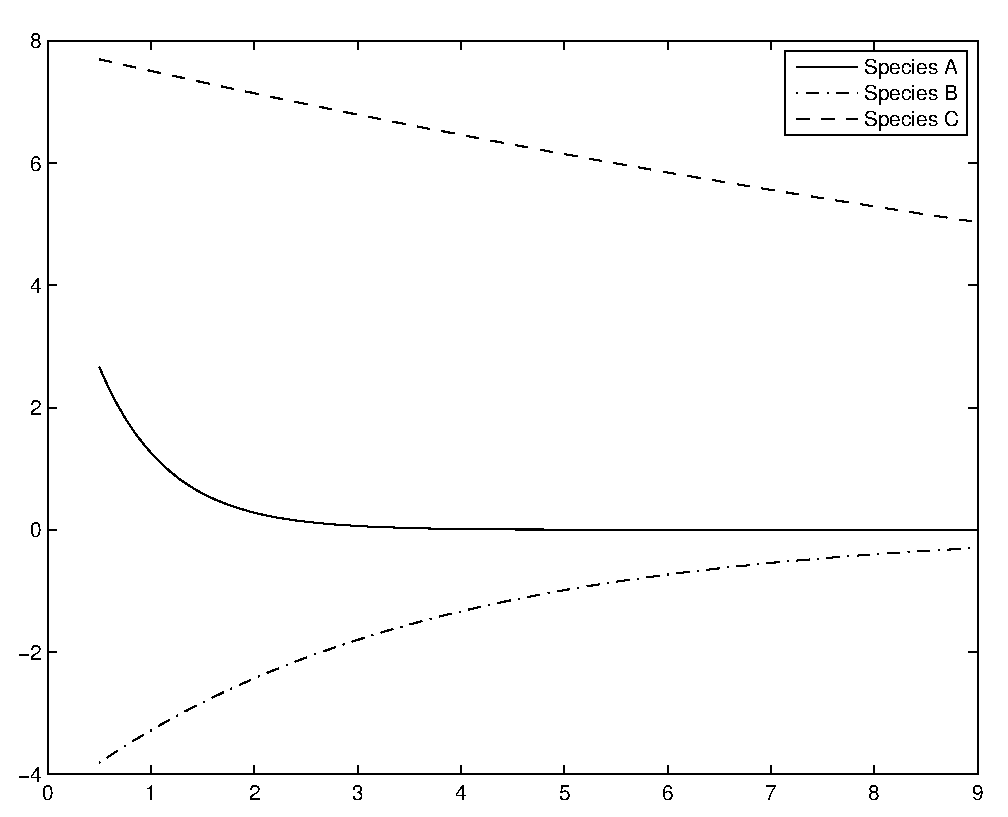
\epsfig{file=Chapra15p10altplot2.eps, width=3.in}
\caption{Chapra 15.10 Alternate}
\end{center}
\end{figure}
\clearpage

\begin{figure}[htb!]
\begin{center}
%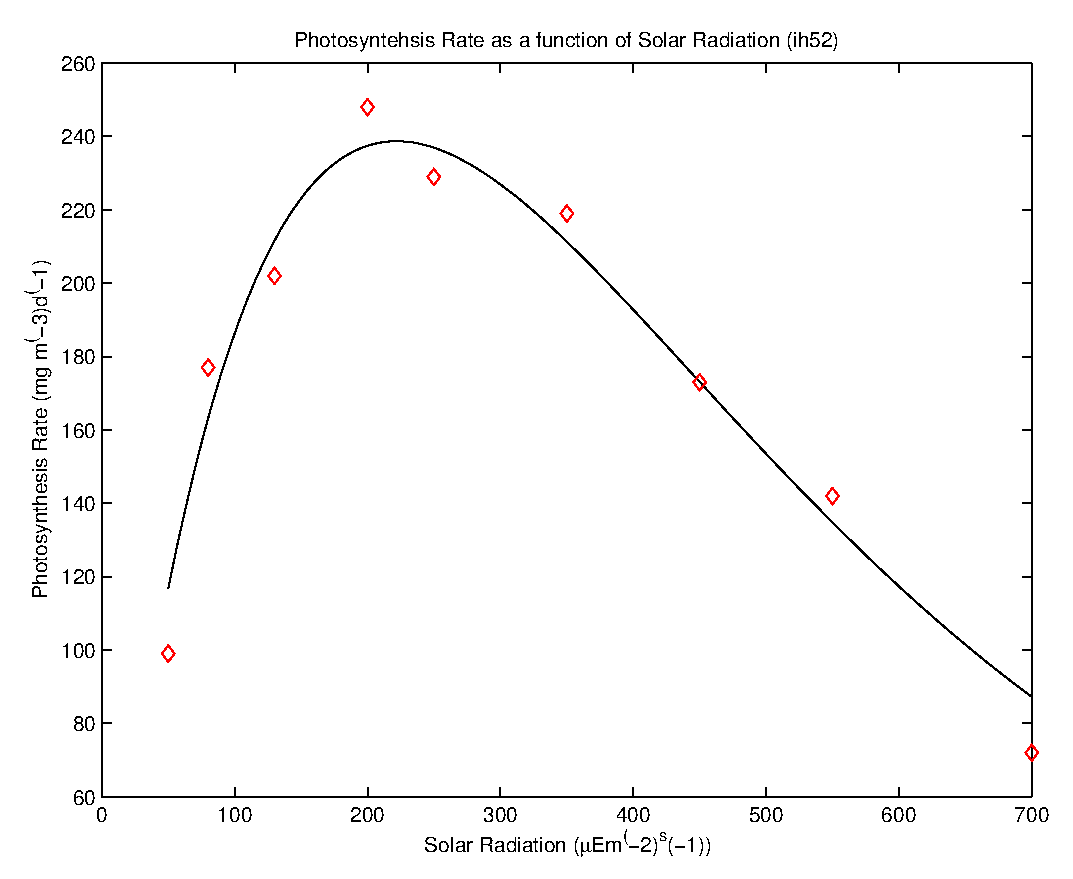
\epsfig{file=Chapra15p11plot.eps, width=4in}
\caption{Chapra 15.11}
\end{center}
\end{figure}

\begin{figure}[htb!]
\begin{center}
%\epsfig{file=Chapra15p14bplot.eps, width=3.1in} ~
%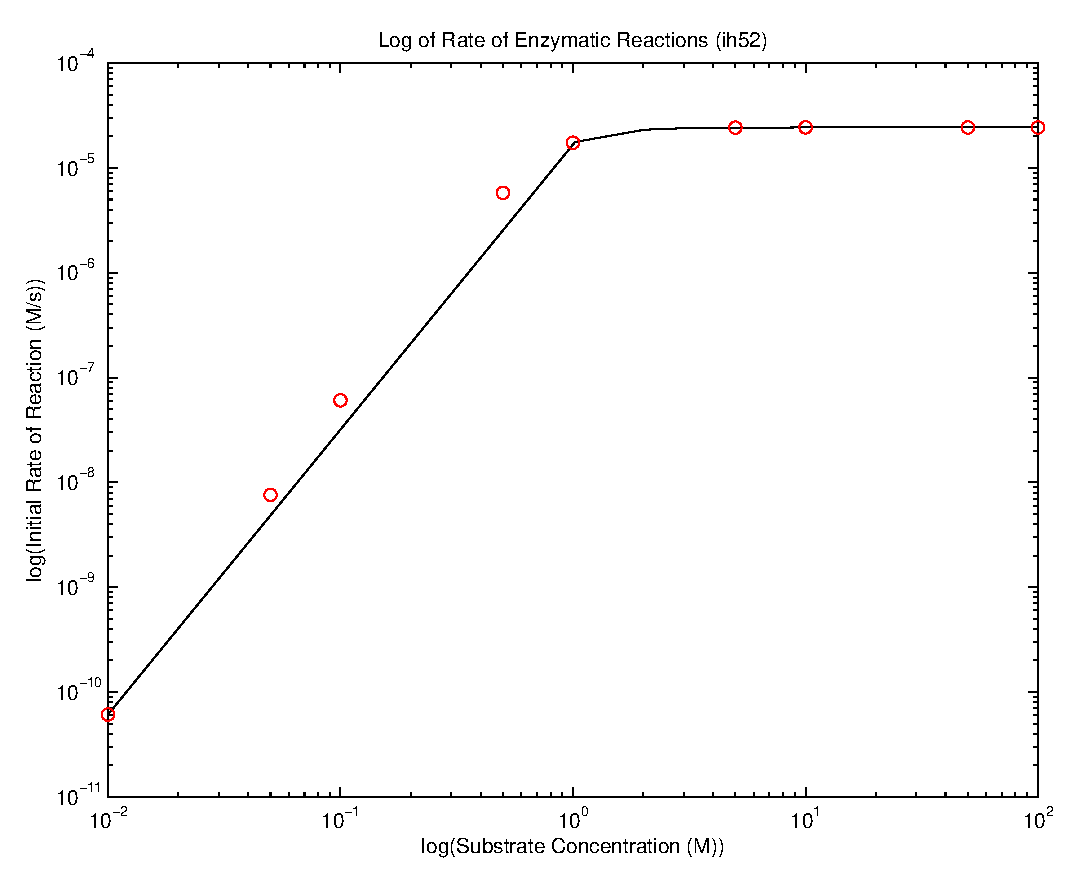
\epsfig{file=Chapra15p14blogplot.eps, width=3.1in}
\caption{Chapra 15.14}
\end{center}
\end{figure}

\end{document}

% LocalWords:  
